\hypertarget{version_8h}{
\section{Dokumentacja pliku /home/pawel/Dokumenty/Uczelnia/grupappz/Source/Ass8-server/version.h}
\label{version_8h}\index{/home/pawel/Dokumenty/Uczelnia/grupappz/Source/Ass8-server/version.h@{/home/pawel/Dokumenty/Uczelnia/grupappz/Source/Ass8-server/version.h}}
}


Ten wykres pokazuje, które pliki bezpośrednio lub pośrednio załączają ten plik:\nopagebreak
\begin{figure}[H]
\begin{center}
\leavevmode
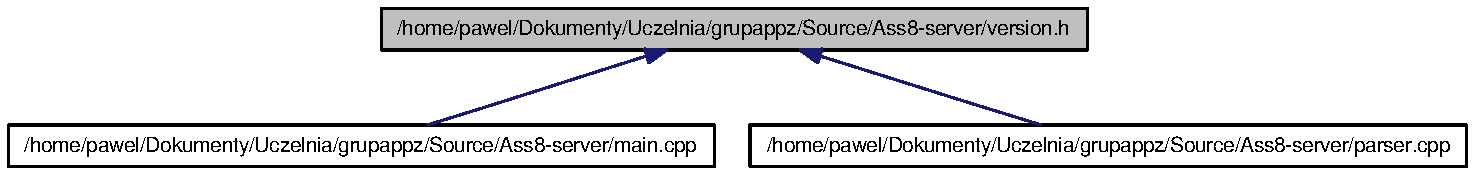
\includegraphics[width=372pt]{version_8h__dep__incl}
\end{center}
\end{figure}
\subsection*{Przestrzenie nazw}
\begin{CompactItemize}
\item 
namespace \hyperlink{namespace_auto_version}{AutoVersion}
\end{CompactItemize}
\subsection*{Definicje}
\begin{CompactItemize}
\item 
\#define \hyperlink{version_8h_0e86d046ea87587e402d375c6b0927c6}{RC\_\-FILEVERSION}~0,3,16,112
\item 
\#define \hyperlink{version_8h_4763e81d3c29ec0fab79225d3ec3f1a2}{RC\_\-FILEVERSION\_\-STRING}~\char`\"{}0, 3, 16, 112$\backslash$0\char`\"{}
\end{CompactItemize}


\subsection{Dokumentacja definicji}
\hypertarget{version_8h_0e86d046ea87587e402d375c6b0927c6}{
\index{version.h@{version.h}!RC\_\-FILEVERSION@{RC\_\-FILEVERSION}}
\index{RC\_\-FILEVERSION@{RC\_\-FILEVERSION}!version.h@{version.h}}
\subsubsection[{RC\_\-FILEVERSION}]{\setlength{\rightskip}{0pt plus 5cm}\#define RC\_\-FILEVERSION~0,3,16,112}}
\label{version_8h_0e86d046ea87587e402d375c6b0927c6}




Definicja w linii 24 pliku version.h.\hypertarget{version_8h_4763e81d3c29ec0fab79225d3ec3f1a2}{
\index{version.h@{version.h}!RC\_\-FILEVERSION\_\-STRING@{RC\_\-FILEVERSION\_\-STRING}}
\index{RC\_\-FILEVERSION\_\-STRING@{RC\_\-FILEVERSION\_\-STRING}!version.h@{version.h}}
\subsubsection[{RC\_\-FILEVERSION\_\-STRING}]{\setlength{\rightskip}{0pt plus 5cm}\#define RC\_\-FILEVERSION\_\-STRING~\char`\"{}0, 3, 16, 112$\backslash$0\char`\"{}}}
\label{version_8h_4763e81d3c29ec0fab79225d3ec3f1a2}




Definicja w linii 25 pliku version.h.